La amplitud es el desplazamiento máximo desde la posición de equilibrio. Se representa con la letra $A$.

La amplitud puede ser hacia arriba o hacia abajo con respecto a la posición de equilibrio.

En el eje de desplazamiento el límite superior se denomina $H$ y el inferior $L$.

{
\centering
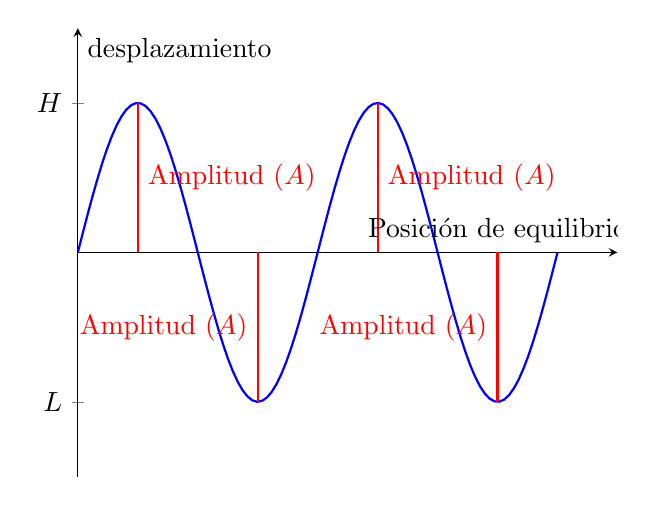
\begin{tikzpicture}
  \begin{axis}[
    xmin=-0,xmax=4.5*pi,
    ymin=-1.5,ymax=1.5,
    axis lines=middle,
    xtick={0},
    ytick={-1,1},yticklabels={$L$,$H$},
    ylabel = desplazamiento,
    ]

    % Funcion senoidal
    \addplot[color=blue,samples=100,domain=0:4*pi,thick]{sin(deg(x))};

    % Amplitud
    \draw[red,thick] (axis cs:pi/2,0) -- (axis cs:pi/2,1) node[pos=0.5,right] {Amplitud ($A$)};
    \draw[red,thick] (axis cs:3*pi/2,0) -- (axis cs:3*pi/2,-1) node[pos=0.5,left] {Amplitud ($A$)};
    \draw[red,thick] (axis cs:5*pi/2,0) -- (axis cs:5*pi/2,1) node[pos=0.5,right] {Amplitud ($A$)};
    \draw[red,thick] (axis cs:7*pi/2,0) -- (axis cs:7*pi/2,-1) node[pos=0.5,left] {Amplitud ($A$)};


    % Posicion de equilibrio
    \node[above] at (axis cs:7*pi/2,0) {Posición de equilibrio};

    % Label y
    % \node[right,rotate=90] at (axis cs:0,0) {desplazamiento};
  \end{axis}
\end{tikzpicture}
}

Para calcular la amplitud se puede hacer uso de los límites superior $(H)$ e inferior $(L)$ en el eje de desplazamiento $y$. Hay dos formas:

\subsubsection{Promedio de la resta de ambos límites}

Consiste en restar los límites y dividir entre dos.

\[
  A=\dfrac{H-L}{2}
\]

Adicionalmente se puede determinar el punto central. Hay dos formas:

Con respecto al límite superior $H$:

\[
  \text{punto central}=H-A
\]

Con respecto al límite inferiro $L$:

\[
  \text{punto central}=L+A
\]

\subsubsection{Promedio de la suma de ambos límites}

Consiste en obtener el promedio de los límites y determinar la diferencia entre los límites y el promedio.

\[
  \text{punto central} = \dfrac{H+L}{2}
\]

Luego se realiza una diferencia para hallar la amplitud $A$. Hay dos formas:

Con respecto al límite superior $H$:

\[
  A = H - \text{punto central}
\]

Con respecto al límite inferior $L$:

\[
  A = \text{punto central} - L
\]
